%********************************************************************************
\documentclass[11pt,subeqn]{article}

%-------------------------------------------------------------------------------
%--- PACKAGES
%-------------------------------------------------------------------------------
\usepackage{url}
\usepackage{longtable}
\usepackage{booktabs}
\usepackage{bold-extra}
\usepackage{rotating}
\usepackage{dcolumn}
\usepackage{color}
\pagecolor{white}
\usepackage{pdfpages}
\usepackage{lastpage}
\usepackage{lscape}
\usepackage{lineno}
\usepackage{setspace}
\usepackage{amsmath}
\usepackage{amssymb}
\usepackage{breqn}
\usepackage{appendix}
\usepackage{natbib}
\usepackage[capposition=top]{floatrow}
\usepackage{graphicx}
\usepackage{epsfig}
\usepackage{epstopdf}
\usepackage{multirow}
\usepackage{titletoc}
\usepackage{wrapfig}
\usepackage{blindtext}
\usepackage{subcaption}
\usepackage{subfloat}
\usepackage{xr}
\externaldocument{BentancorClarke_AdolescentFertility}

%-------------------------------------------------------------------------------
%--- SPECIFICATIONS (MARGINS, TOC, BIBLIO)
%-------------------------------------------------------------------------------
\setlength\topmargin{-0.375in}
\setlength\textheight{8.8in}
\setlength\textwidth{5.8in}
\setlength\oddsidemargin{0.4in}
\setlength\evensidemargin{-0.5in}


\bibliographystyle{abbrvnat}
\bibpunct{(}{)}{;}{a}{,}{,}



\titlecontents{section}
[0pt]
{}%
{\contentsmargin{0pt}
    \thecontentslabel\enspace%
    }
{\contentsmargin{0pt}}
{\titlerule*[.5pc]{.}\contentspage}
[]

\renewcommand\figurename{Appendix Figure}
\renewcommand\tablename{Appendix Table}
\renewcommand\thesection{\Alph{section}}



%-------------------------------------------------------------------------------
%--- FRONT PAGE
%-------------------------------------------------------------------------------
\begin{document}
\begin{spacing}{1.4}

\begin{center}
\textbf{ONLINE APPENDICES} \\
\vspace{4mm}
From the paper: \\
\vspace{6mm}
{\large \textsc{Assessing Plan B: 
The Effect of the Morning After Pill on Children and Women}} \\
Damian Clarke and Andrea Bentancor
\end{center}

\tableofcontents


%-------------------------------------------------------------------------------
%--- MAIN CONTENTS
%-------------------------------------------------------------------------------
\setlength\parindent{0.25in}
\setlength\parskip{0.25in}


\newpage
\section{Data Appendix: Births and Deaths}
Population data from Chile comes from two main sources.  The first is vital 
statistics data, recording births and fetal deaths which are provided by the 
Ministry of Health of the Government of Chile (MINSAL).  This data provides 
microdata records covering greater than 99\% of all births and fetal deaths 
reported in aggregate data \citep{Bharadwajetal2013} in the country.  Each 
entry records the occurrence of a birth or fetal death, characteristics of the 
mother (and if present father) including her age, education, and muncipality of 
residence, as well as a number of charactersitics of the birth (including birth 
weight, gender, gestation and birth order) or the fetal death (weeks of 
gestation, birth order, ICD-10 code\footnote{The ICD (or Internation 
Classification of Disease) code is a standard set of codes which classify deaths 
according to their cause. These are used worldwide to facilitate classification 
and generation of national mortality statistics. The ICD-10 has been in use in
Chile to classify fetal (and all) deaths since 1997 \citep{INE2014}.}). These 
data have been collected and reported in Chile since 1982, and, at the time of 
writing, are publicly available online up to the year 2012 at the following url: 
\texttt{http:\/\/www.deis.cl\/?p=1020}.  These vital statistics data for birth 
and fetal deaths thus provide data on all pregnant women in the country who 
either give live birth, have a birth leading to fetal death or who miscarry in 
any hospital in the country. 

Data on all women of reproductive age comes from the National Institute of 
Statistics of Chile (INE). The INE provides estimations of the number of women 
of each age living in each municipality in each year.  These estimates are based 
on the decennial census, as well as net migration each year, and vital 
statistics on all births and deaths occurring to residents in the municipality 
\citep{INE2014}.  These two sources of data provide information on the number
of women of fertile age living in each municipality, and the number of women
pregnant in each municipality during the time period of interest.  They can be
merged at the level of the municipality, resulting in counts of total number of
births and non-pregnant women, and also the calculation of municipal-level rates
of pregnancy (births/total women), and fetal deaths (deaths/total births).

Appendix tables \ref{strucTab} and \ref{reshapeTab} provide an excerpt of the
structure of the data constructed using MINSAL vital statistics and INE 
population records.  Municipal level data of population and total births are
collected for each municipality, year and age group, and the number of 
non-pregnant women is calculated by subtracting pregnant women from the total
female population of this age (Appendix table \ref{strucTab}).  From this
table rates and counts of births are known and OLS regressions can be run.  In 
order to run a weighted binary regression, this table can be reshaped, to form
records of the number of pregnant and non-pregnant women in each municipality,
year and age group (Appendix table \ref{reshapeTab}).  In both cases, the data
are matched at the level of the municipality, so all birth and population 
records are successfully matched.

\end{spacing}
\begin{spacing}{1}
\begin{table}[htpb!]
\begin{center}
\caption{Birth and Population Data (18 year olds)}
\label{strucTab}
\begin{tabular}{lccccc} \toprule
Comuna & Year & Population & Pregnant & Not Pregnant & Rate \\ \midrule
Arica & 2009 & 1575 & 119 & 1456 & 0.076 \\
Arica & 2010 & 1579 & 118 & 1461 & 0.075 \\ 
Arica & 2011 & 1534 & 116 & 1418 & 0.076 \\ \bottomrule
\multicolumn{6}{p{11.2cm}}{\begin{footnotesize}\textsc{Note:} Column 3 is from INE, 
column 4 from MINSAL. Non-pregnancies in Column 5 are calculated from birts and
total women (Column 3$-$Column 4), and the rate is calcualted by taking the ratio
of pregancies over total women (Column 4/Column 3).\end{footnotesize}}
\end{tabular}
\end{center}
\end{table}

\begin{table}[htpb!]
\begin{center}
\caption{Reshaped Data for Analysis (18 yo)}
\label{reshapeTab}
\begin{tabular}{lccc} \toprule
Comuna & Year & Pregnant & Weight \\ \midrule
Arica & 2009 & 1 & 119 \\
Arica & 2009 & 0 & 1456 \\
Arica & 2010 & 1 & 118 \\
Arica & 2010 & 0 & 1461 \\
Arica & 2011 & 1 & 116 \\
Arica & 2011 & 0 & 1418 \\ \bottomrule
\end{tabular} \\
\end{center}
\end{table}
\end{spacing}
\begin{spacing}{1.4}

%-------------------------------------------------------------------------------
We observe 1,605,300 live births and 13,063 fetal deaths occurring to 15-49 year 
old women from 2006-2012.  Appendix figure \ref{TEENfig:ageHist} plots the 
distribution of mother's age at birth in Chile over the period of study, while
figure \ref{TEENfig:ageHistD} plots the distribution of fetal deaths by ages of
the woman.  For births, the distribution is approximately multi-modal, with a 
peak for women in their late teens and early 20s, and another peak in the late 
20s.  As in the USA, the rate of fetal deaths are highest among teenage and 
older women \citep{MacDormanGregory2015}, with the absolute number in Chile 
being highest among young women.

\begin{figure}[htpb!]
\begin{center}
\caption{Frequency of Births by Mother's Age: Chile 2006-2012}
\label{TEENfig:ageHist}
\includegraphics[scale=0.44]{../Figures/ageDistBirths.pdf} 
\end{center}
\end{figure}

\begin{figure}[htpb!]
\begin{center}
\caption{Frequency of Fetal Deaths by Mother's Age: Chile 2006-2012}
\label{TEENfig:ageHistD}
\includegraphics[scale=0.44]{../Figures/ageDistDeaths.pdf} 
\end{center}
\vspace{-4mm}
\floatfoot{\textsc{Notes to Appendix figures \ref{TEENfig:ageHist}-
\ref{TEENfig:ageHistD}}: 
Sample consists of all births and fetal deaths (respectively) occurring in Chile
between the years of 2006-2012.  Data comes from the Ministry of Health of the
Government of Chile's vital statistics data.}
\end{figure}

The population of fertile-aged women in Chile during this period was 
approximately 4 million\footnote{According to the 2002 census, the population
of Chile was 15,116,435, of which 50.7\% were women.  The most recent estimates
from INE are 17,556,815, and 50.5\% respectively.}  Over the entire period 
2006-2012, 28,196,700 fertile aged women were exposed (4 million women in 7 
years).  Appendix figure \ref{TEENfig:Pregtime} displays pregnancy rates by
age-group over the period of study, calculated from MINSAL vital statistics
and INE population data.  These figures are virtually indistinguishable from
rates published in aggregate data by MINSAL \citep{MINSAL2013}.\footnote{For
example, The Ministry of Health reports that the rate of pregnancy per 1,000
women aged 15-19 over the same period was: 51.0 per 1,000 in 2006, 53.4/1,000
in 2007, 54.9/1,000 in 2008, 54.3/1,000 in 2009, 52.0/1,000 in 2010, 
50.4/1,000 in 2011, and 48.6/1,000 in 2012.}  A similar figure for rates of
birth and death for the entire population under study is presented in the
body of the paper (figure \ref{TEENfig:BirthDeath}).

\begin{figure}[htpb!]
\begin{center}
\caption{Pregancies by Age Group and Time}
\vspace{-5mm}
\label{TEENfig:Pregtime}
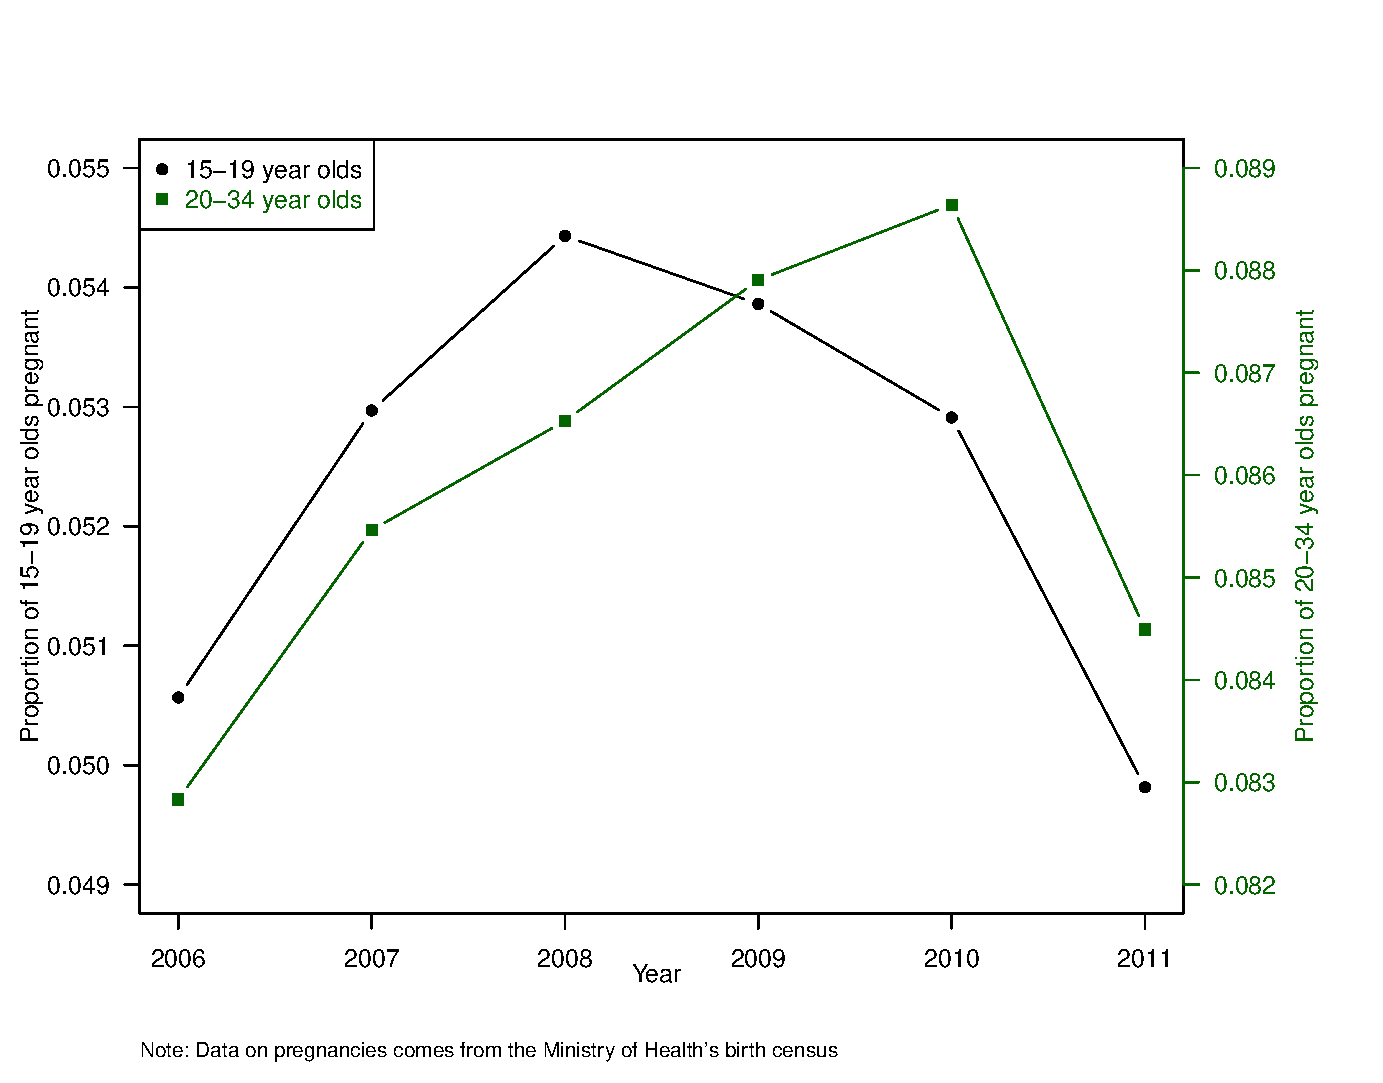
\includegraphics[scale=0.54]{../Figures/Births.eps} 
\end{center}
\end{figure}


\clearpage
\renewcommand\thesection{\Alph{section}}
\setlength\parindent{0.25in}
\setlength\parskip{0.25in}

\section{Data Appendix: Distance to Treatment}
Spillover analysis in section \ref{TEENsscn:spillover} of the paper requires
data on the distance of each non-treatment municipality to the nearest 
treatment municipality.  Principal measures of distance from treatment is 
calculated by using GIS software to take a Euclidean distance from the 
centroid of non-treatment municipalities, to the centroid of the nearest 
municipality which did offer the morning after pill in each year under 
study.\footnote{In order to calculate distances, the official map shape file
from the Chilean Library of Congress was consulted, which available on the
web at \texttt{http://siit2.bcn.cl/mapas_vectoriales}.}  The distribution of
distances from each non-treatment municipality to its nearest treatment 
municipality in kilometres is presented in Appendix figure \ref{dist}.

\begin{figure}[htpb!]
\includegraphics[scale=0.55]{../Figures/EuclideanDistance.eps}
\caption{Simple Distance to Treatment}
\label{dist}
\floatfoot{\textsc{Notes to figures \ref{dist}}: 
Histogram presents the distance from each municipality where the pill
was not available to the closest pill municipality in the years 2009-2011.
Distances over 150 km have been omitted for clarity.  Less than 1.5\% of 
non-pill municipalities are greater than 150km from the nearest pill 
municipality.}
\end{figure}


As a robustness check, alternative distance measures were also used.
Firstly, we collated the shortest distance over roads from non-teatment to 
treatment municipalities.  This was calculated using repeated calls to the 
Google Distance Matrix API\footnote{Full details can be found at:
\url{https://developers.google.com/maps/documentation/distancematrix/\#api\_key}.
I have made the computational routine used available on the web at:
\url{https://github.com/damiancclarke/spillovers/blob/master/source/distCalc/queryDist.py}.}, 
which finds the shortest path over roads.  In the case of Chile, this requires 
calculating the distances between all 346 municipalities ($346^2/2=59,858$ 
distance pairs) in each year.  Secondly, rather than distance in 
kilometres, as in Euclidean or road distance, a measure of travel \emph{time} 
was calculated.  As a proxy for total travel time, travel time by car was 
caclulated between areas.  This was similarly generated using calls to Google 
Maps, resulting in one value for each municipality pair (see example in Appendix
Figure \ref{googdist}).  In each case ``distance to treatment'' is then the 
minimum value to the nearest treatment area, which varies by municipality and 
year.  Appendix Figure \ref{altdist} displays the distribution of alternative
distance measures for shortest distance over roads, and travel time in car.

\begin{figure}[htpb!]
\includegraphics[scale=0.7]{../Figures/mapDistance.png}
\caption{Distance based on googlemaps}
\label{googdist}
\end{figure}

\begin{figure}[htpb!]
\begin{center}
\caption{Alternative Measures of Distance to Treatment}
\label{altdist}
\begin{subfigure}{.5\textwidth}
  \centering
  \includegraphics[scale=0.32]{../Figures/TravelTime.eps}
  \caption{Travel time by vehicle}
  \label{travelTime}
\end{subfigure}%
\begin{subfigure}{.5\textwidth}
  \centering
  \includegraphics[scale=0.32]{../Figures/RoadDistance.eps}
  \caption{Distance over roads}
  \label{roadDist}
\end{subfigure}
\end{center}
\vspace{-4mm}
\floatfoot{\textsc{Notes to figures \ref{altdist}}: 
Histograms present the distance from each municipality where the pill
was not available to the closest pill municipality in the years 2009-2011.
Distances over 150 km (minutes) have been omitted for clarity.  In each 
case, less than 1.5\% of non-pill municipalities are greater than 150km 
(minutes) from the nearest pill municipality.}
\end{figure}



These alternative measures of distance do not majorly affect the quantitative 
implication of findings reported in the paper.  Appendix tables \ref{altdist1}
and \ref{altdist2} replicate table \ref{TEENtab:Spillover} from the paper,
replacing Euclideand distance with distance over roads, or travel time in 
car. Results from both tables suggest a treatment effect of approximately 
-0.075 once accounting for spillovers of 30 minutes travel time or 30km of 
distance respectively, following the spillover methodology outlined in the
paper.







\clearpage
\section{Time-Varying Municipality and Region Controls}
Time-varying municipal controls such as education and health spending, and the
number of females working in public government is downloaded from the National
System of Municipal Information (SINIM).  This provides data as far back as
2005, and is freely available for download online at
\url{http://www.sinim.gov.cl/indicadores/busq_serie.php}.

Data on municipal elections, mayor's gender, party and vote share is accessed
from the Electoral Service of Chile (SERVEL).  This provides all electoral
results from municipal elections for the full time period of this study.  Raw
data is available online at 
\url{http://www.servel.cl/ss/site/mobile/padron_electoral_comunal_por_ano_informe_comunal_anual.html}
or processed as one line per municipality at the data page of the author's
website linked to above.

Finally, we calculate data for alternative contraceptive use based on
a series of regionally representative surveys collected every 3 years beginning
in 1994.  The National Survey of Youth asks respondents whether they use any 
method of contraception in both their first and most recent sexual activity.  
In the case that they did not use a condom, they are asked whether this is 
because they did not have access.  Based on this survey, access to condom is
calculated as an additional time-varying control.  However, it should be noted
that this variable can only be calculated at the level of the region (one 
level above the municipality), given that this survey is not representative at 
the level of the municipality.  Once again, processed data and processing 
scripts are made available at the data section of the author's site, and, if 
desired, raw data is available on the web: 
\url{http://extranet.injuv.gob.cl/Encuesta_Nacional_de_la_Juventud/contenido/index.php}.




\clearpage
\section[Additional Details of the Emergency Contraceptive Reform]{The Chilean 
Legislative Environment and the Adoption of Emergency Contraception}
\label{TEENscn:applegislate}
Discussions surrounding the introduction of emergency contraception in Chile
have taken place since at least 1996, when the Chilean Institute of 
Reproductive Medicine (ICMER for its initials in Spanish) proposed the use of
this method to avoid undesired pregnancies in a country where abortion was
entirely outlawed \citep{Dides2009}.  However, the first legislative attention
given to this matter occurred when the aforementioned (see section 
\ref{TEENsscn:Chile}) Institute of Public Health emitted a resolution allowing
for the production and sale of `Postinol', a drug containing levonogestrel by a
Chilean laboratory in 2001.  The Constitionality of this was quickly 
challenged, and the drug was prohibited by the Supreme Court.

The emergency contraceptive pill again entered legislative attention in 2004,
following the Ministry of Health's publication of a guide suggesting that 
emergency contraception be used following cases of rape.  Following this in 
2005, the Subsecretary of Health Dr.\ Antonio Infante announced that emergency
contraception would be freely available to \emph{all} women who requested it,
however the President of Chile and the Ministry of Health later declared that
this was not the case, leading to removal of the Subsecretary from office.

In November of 2005, the Supreme Court of Chile provided the first 
constitutional support for the emergency contraceptive pill, voting 5-0 to
reverse the decision taken in 2001, allowing emergency contraception to be
provided in the case that the mother's life was in danger.  Once again however,
this finding was challenged shortly thereafter.  The same non-governmental 
institution which had earlier raised a case against ICMER, now challenged the 
private commercial laboratory in charge of producing and distributing the drug.  
However, before this case could reach court, this laboratory voluntarily gave 
up their license to produce the drug, in a three line statement issued by the
General Director of the company on February 14, 2006 \citep{CasasBecerra2008}.

In the same year, a group of 36 parliamentary deputies from conservative 
parties raised a case with the Constitional Tribunal, claiming that the 
provision of the emergency contraceptive pill contravened the ``National Laws
for the Regulation of Fertility'', a set of rules issued by the Ministry of
Health.  This case was only resolved in 2008, with the Constitional Tribunal's
finding in favour of this group, hence making illegal any provision by 
hospitals or health centres controlled by the Ministry of Health (and hence
under the jurisdiction of the National Fertility Laws).  Fundamentally however,
this left the door open for Municipal health centres to distribute the pill
freely to women.  These Municipal Health Centres are run under the directive
of the elected mayor of each Municipality, leaving all remaining legislation 
regarding the distribution of the pill up to the 346 mayors in Chile.

In this study we study the period surrounding this 2008 legislation as the 
cutoff of interest.  However, even after this finding the emergency 
contraceptive pill has not been far from legislative action, with a number of
other cases raised.  These cases never entirely threatened the continuity of
supply of the morning after pill by municipalities, however did cause some
confusion for mayors and municipal health bodies in determining whether or not
they were legally allowed to prescribe the contraceptive.  These cases also
resulted in the passing of a number of laws and standards.  Most importantly,
they resulted in national Law 20.418 which ``creates standards for information,
guidance and regulatory services in fertility'' (author's translation), and 
the passing of a decree on March 3, 2013, which makes obligatory the provision
of the morning after pill to women of any age in any health centre in Chile.  
This became operative on May 28, 2013, meaning that---at least officially---%
there are no longer any restrictions in place in the country.




\clearpage
\section{Alternative Specifications}
\begin{table}[!htbp] \centering
\caption{The Effect of the EC Pill on Birth Rates}
\label{TEENtab:aggregateASFR}
\begin{tabular}{@{\extracolsep{5pt}}lcccc}
\\[-1.8ex]\hline \hline \\[-1.8ex] 
& Birth& Birth& Birth& Birth\\
& Rate & Rate & Rate & Rate \\
&(1)&(2)&(3)&(4) \\ \hline
\multicolumn{5}{l}{\textbf{
\noindent Panel A: All Women}} \\
Emergency Contraceptive Pill     &$-$1.193$^{***}$&$-$2.247$^{***}$&$-$1.562$^{***}$&$-$1.721$^{***}$\\
            &[0.425]&[0.489]&[0.524]&[0.620]\\
 & & & & \\
Observations&2,210&2,210&2,210&2,210\\
Mean Birth Rate&53.87&53.87&53.87&53.87\\
 & & & & \\
\multicolumn{5}{l}{\noindent \textbf{
Panel B: 15-19 year olds}} \\
Emergency Contraceptive Pill&$-$3.811$^{***}$&$-$4.546$^{***}$&$-$2.795$^{**}$&$-$3.536$^{**}$\\
            &[0.714]&[1.179]&[1.218]&[1.538]\\
 & & & & \\
Observations&2,205&2,205&2,205&2,205\\
Mean Birth Rate&52.00&52.00&52.00&52.00\\
 & & & & \\
\multicolumn{5}{l}{\noindent \textbf{
Panel C: 20-34 year olds}} \\
Emergency Contraceptive Pill&$-$2.491$^{***}$&$-$3.277$^{***}$&$-$2.273$^{**}$&$-$2.452$^{**}$\\
            &[0.762]&[0.891]&[0.938]&[1.116]\\
 & & & & \\
Observations&2,210&2,210&2,210&2,210\\
Mean Birth Rate&85.49&85.49&85.49&85.49\\
 & & & & \\
\multicolumn{5}{l}{\noindent \textbf{
Panel B: 35-49 year olds}} \\
Emergency Contraceptive Pill&0.240&$-$0.586&$-$0.401&$-$0.106\\
            &[0.274]&[0.411]&[0.455]&[0.600]\\
 & & & & \\
Observations&2,210&2,210&2,210&2,210\\
Mean Birth Rate&21.40&21.40&21.40&21.40\\
\hline \\[-1.8ex] 
{\small Year \& Comuna FEs}             &Y&Y&Y&Y \\
{\small Municipal-Specific Linear Trends}& &Y&Y&Y \\
{\small Time Varying Controls}           & & &Y&Y \\
{\small Spillovers}                      & & & &Y \\
\hline \hline \\[-1.8ex]
\multicolumn{5}{p{12.8cm}}{\begin{footnotesize}
\textsc{Notes:} Each panel presents population-weighted
 difference-in-difference results for a regression of 
age-specific fertility rates (ASFR) on the EC reform for
 the age group in
 each municipality.  ASFR is defined as the number of   
births per 1,000 women.  In the case of all women, this 
is called the General Fertility Rate (GFR). All models  
are estimated by OLS, and each municipality is          
weighted by the population of women. Time varying       
controls included in the regression consist of party    
dummies for the mayor in power, the mayor's gender, the
 vote margin of the mayor, the percent of girls out of  
highschool, education spending spending by both the     
municipality and the Ministry of Education, total       
health spending and health spending on staff and        
training, the percent of female heads of households     
living below the poverty line, the percent of female    
workers in professional positions in the Municipality,  
and condom availability (measured at the level of the   
region). Standard errors are clustered at the level of  
the municipality.
$^{*}$p$<$0.1; $^{**}$p$<$0.05; $^{***}$p$<$0.01\end{footnotesize}}
\normalsize\end{tabular}\end{table}

\begin{table}[htpb!] \centering
\caption{The Effect of the EC Pill on Fetal Death Rates}
\label{TEENtab:DeathOLS}
\begin{tabular}{@{\extracolsep{5pt}}lccc}\\[-1.8ex]
\hline\hline\\[-1.8ex]
& All    & Early     & Late      \\
& Deaths & Gestation & Gestation \\ \midrule
\multicolumn{4}{l}{\noindent \textbf{
Panel A: All Women}} \\
Emergency Contraceptive Pill &0.313&$-$0.031&0.281\\
&[0.645]&[0.330]&[0.517]\\
& & & \\
Observations&2,189&2,189&2,189\\
Mean (fetal deaths/live birth)&8.14&2.40&4.76\\
&&&\\
\multicolumn{4}{l}{\noindent \textbf{
Panel B: 15-19 year olds}} \\
Emergency Contraceptive Pill &0.994&$-$1.344$^{*}$&2.175\\
&[1.674]&[0.730]&[1.467]\\
& & & \\
Observations&2,157&2,157&2,157\\
Mean (fetal deaths/live birth)&8.02&2.42&4.83\\
&&&\\
\multicolumn{4}{l}{\noindent \textbf{
Panel C: 20-34 year olds}} \\
Emergency Contraceptive Pill &0.378&0.394&0.071\\
&[0.691]&[0.350]&[0.630]\\
& & & \\
Observations&2,184&2,184&2,184\\
Mean (fetal deaths/live birth)&7.37&2.21&4.35\\
&&&\\
\multicolumn{4}{l}{\noindent \textbf{
Panel C: 35-49 year olds}} \\
Emergency Contraceptive Pill &$-$0.540&$-$0.227&$-$0.512\\
&[2.032]&[1.512]&[1.400]\\
& & & \\
Observations&2,159&2,159&2,153\\
Mean (fetal deaths/live birth)&11.47&3.21&6.23\\
\hline \hline \\[-1.8ex]
\multicolumn{4}{p{10.2cm}}{\begin{footnotesize}          
\textsc{Notes:} Each panel presents weighted difference-
in-difference results for a regression of the fetal      
death rate (deaths per 1,000 live births) on the EC      
reform for the age group in question. All models are     
estimated by OLS, and each municipality is weighted by   
the number of live births. All regressions include the   
controls documented in table \ref{TEENtab:aggregateASFR}.
Standard errors are clustered at the level of the        
municipality.
$^{*}$p$<$0.1; $^{**}$p$<$0.05; $^{***}$p$<$0.01;\end{footnotesize}}
\normalsize\end{tabular}\end{table}

\begin{table}[!htbp] \centering
\caption{The Effect of the EC Pill on log Births}
\label{TEENtab:aggregateLog}
\begin{tabular}{@{\extracolsep{5pt}}lcccc}
\\[-1.8ex]\hline \hline \\[-1.8ex] 
& ln(Birth) & ln(Birth) & ln(Birth) & ln(Birth) \\
&(1)&(2)&(3)&(4) \\ \hline
\multicolumn{5}{l}{\textbf{
\noindent Panel A: All Women}} \\
Emergency Contraceptive Pill&$-$0.026$^{***}$&$-$0.046$^{***}$&$-$0.029$^{***}$&$-$0.029$^{**}$\\
            &[0.008]&[0.010]&[0.010]&[0.012]\\
 & & & & \\
Observations&2,210&2,210&2,210&2,210\\
Mean of ln(Births+1) &7.37&7.37&7.37&7.37\\
 & & & & \\
\multicolumn{5}{l}{\noindent \textbf{
Panel B: 15-19 year olds}} \\
Emergency Contraceptive Pill&$-$0.113$^{***}$&$-$0.089$^{***}$&$-$0.055$^{***}$&$-$0.064$^{***}$\\
            &[0.012]&[0.020]&[0.020]&[0.024]\\
 & & & & \\
Observations&2,205&2,205&2,205&2,205\\
Mean of ln(Births+1) &5.46&5.46&5.46&5.46\\
 & & & & \\
\multicolumn{5}{l}{\noindent \textbf{
Panel C: 20-34 year olds}} \\
Emergency Contraceptive Pill&$-$0.009&$-$0.036$^{***}$&$-$0.024$^{**}$&$-$0.025$^{*}$\\
            &[0.009]&[0.011]&[0.012]&[0.014]\\
 & & & & \\
Observations&2,210&2,210&2,210&2,210\\
Mean of ln(Births+1) &7.02&7.02&7.02&7.02\\
 & & & & \\
\multicolumn{5}{l}{\noindent \textbf{
Panel B: 35-49 year olds}} \\
Emergency Contraceptive Pill&0.000&$-$0.032&$-$0.022&$-$0.010\\
            &[0.012]&[0.020]&[0.021]&[0.026]\\
 & & & & \\
Observations&2,210&2,210&2,210&2,210\\
Mean of ln(Births+1) &5.55&5.55&5.55&5.55\\
\hline \\[-1.8ex] 
{\small Year \& Comuna FEs}             &Y&Y&Y&Y \\
{\small Municipal-Specific Linear Trends}& &Y&Y&Y \\
{\small Time Varying Controls}           & & &Y&Y \\
{\small Spillovers}                      & & & &Y \\
\hline \hline \\[-1.8ex]
\multicolumn{5}{p{13.8cm}}{\begin{footnotesize}
\textsc{Notes:} Each panel presents population       
weighted difference-in-difference results for a       
regression of the log(Births+1) for the age group in  
each  municipality. Specifications are identical to   
table \ref{TEENtab:aggregateASFR}, however logs are  
 used in place of birth rates. Standard errors are    
clustered at the level of the municipality.
$^{*}$p$<$0.1; $^{**}$p$<$0.05; $^{***}$p$<$0.01\end{footnotesize}}
\normalsize\end{tabular}\end{table}

\begin{table}[!htbp] \centering
\caption{The Effect of the EC Pill on Total Births}
\label{TEENtab:aggregate}
\begin{tabular}{@{\extracolsep{5pt}}lcccc}
\\[-1.8ex]\hline \hline \\[-1.8ex] 
& Number& Number & Number & Number \\
& Births& Births & Births & Births \\
&(1)&(2)&(3)&(4) \\ \hline
\multicolumn{5}{l}{\textbf{
\noindent Panel A: All Women}} \\
Emergency Contraceptive Pill&7.623&$-$27.564$^{***}$&$-$20.337$^{***}$&$-$25.936$^{***}$\\
            &[5.720]&[5.242]&[5.954]&[8.511]\\
 & & & & \\
Observations&2,210&2,210&2,210&2,210\\
Mean Number of Births&2632.67&2632.67&2632.67&2632.67\\
 & & & & \\
\multicolumn{5}{l}{\noindent \textbf{
Panel B: 15-19 year olds}} \\
Emergency Contraceptive Pill&$-$8.618$^{***}$&$-$8.519$^{***}$&$-$5.583$^{***}$&$-$7.474$^{***}$\\
            &[1.233]&[1.517]&[1.716]&[2.275]\\
 & & & & \\
Observations&2,205&2,205&2,205&2,205\\
Mean Number of Births&386.14&386.14&386.14&386.14\\
 & & & & \\
\multicolumn{5}{l}{\noindent \textbf{
Panel C: 20-34 year olds}} \\
Emergency Contraceptive Pill&11.605$^{***}$&$-$16.644$^{***}$&$-$12.890$^{***}$&$-$17.893$^{***}$\\
            &[4.173]&[3.621]&[4.257]&[6.101]\\
 & & & & \\
Observations&2,210&2,210&2,210&2,210\\
Mean Number of Births&1833.11&1833.11&1833.11&1833.11\\
 & & & & \\
\multicolumn{5}{l}{\noindent \textbf{
Panel B: 35-49 year olds}} \\
Emergency Contraceptive Pill&4.636$^{***}$&$-$2.401$^{*}$&$-$1.843&$-$0.541\\
            &[1.608]&[1.299]&[1.371]&[1.742]\\
 & & & & \\
Observations&2,210&2,210&2,210&2,210\\
Mean Number of Births&435.78&435.78&435.78&435.78\\
\hline \\[-1.8ex] 
{\small Year \& Comuna FEs}             &Y&Y&Y&Y \\
{\small Municipal-Specific Linear Trends}& &Y&Y&Y \\
{\small Time Varying Controls}           & & &Y&Y \\
{\small Spillovers}                      & & & &Y \\
\hline \hline \\[-1.8ex]
\multicolumn{5}{p{14.2cm}}{\begin{footnotesize}
\textsc{Notes:} Each panel presents population       
weighted difference-in-difference results for a       
regression of the total number of births for the age  
group in each municipality. Specifications are        
identical to table \ref{TEENtab:aggregateASFR},      
however birth weights are replaced by the total number
 of births. Standard errors are clustered             
at the level of the municipality.
$^{*}$p$<$0.1; $^{**}$p$<$0.05; $^{***}$p$<$0.01\end{footnotesize}}
\normalsize\end{tabular}\end{table}

\begin{table}[htpb!] \centering 
  \caption{The Morning After Pill and Pregnancy: Full Covariates} 
  \label{TEENtabPregFull} 
\begin{tabular}{@{\extracolsep{5pt}}lccc} 
\\[-1.8ex]\hline 
\hline \\[-1.8ex] 
 & \multicolumn{3}{c}{Pregnancy} \\ 
\cline{2-4} 
\\[-1.8ex] & 15-19 & 20-34 & 35-49 \\ 
 & year olds & year olds & year olds \\ 
\\[-1.8ex] & \multicolumn{1}{c}{(1)} & \multicolumn{1}{c}{(2)} & \multicolumn{1}{c}{(3)}\\ 
\hline \\[-1.8ex] 

 Morning After Pill & -0.041$^{***}$ & -0.030$^{***}$ & 0.006 \\ 
  & (0.010) & (0.005) & (0.010) \\ 
  & & & \\ 
 Female Mayor & 0.016 & -0.005 & -0.007 \\ 
  & (0.026) & (0.013) & (0.026) \\ 
  & & & \\ 
 Mayor's Support & 0.054 & 0.017 & -0.129 \\ 
  & (0.084) & (0.042) & (0.085) \\ 
  & & & \\ 
 Out of School & -0.004 & -0.001 & -0.001 \\ 
  & (0.003) & (0.001) & (0.003) \\ 
  & & & \\ 
 Total Education Spending & 0.001$^{*}$ & -0.00004 & 0.001$^{**}$ \\ 
  & (0.0003) & (0.0002) & (0.0003) \\ 
  & & & \\ 
 Municipal Education Spending & -0.004$^{***}$ & -0.001$^{**}$ & -0.001$^{**}$ \\ 
  & (0.001) & (0.0003) & (0.001) \\ 
  & & & \\ 
 Health Spending & -0.0002 & 0.0001 & -0.0005 \\ 
  & (0.001) & (0.0003) & (0.001) \\ 
  & & & \\ 
 Health Training & -0.080$^{***}$ & -0.036$^{***}$ & 0.005 \\ 
  & (0.024) & (0.012) & (0.025) \\ 
  & & & \\ 
 Health Staff & 0.001 & 0.001$^{***}$ & -0.0004 \\ 
  & (0.001) & (0.0005) & (0.001) \\ 
  & & & \\ 
 Female Poverty & -0.0004 & -0.0001 & 0.002$^{***}$ \\ 
  & (0.001) & (0.0003) & (0.001) \\ 
  & & & \\ 
 Female Workers & -0.001 & -0.0005 & 0.001 \\ 
  & (0.001) & (0.0004) & (0.001) \\ 
  & & & \\ 
\hline \\[-1.8ex] 
Years $\times$ Municipality & 1,929 & 1,934 & 1,934 \\ 
\hline 
\hline \\[-1.8ex] 
\multicolumn{4}{p{10.8cm}}{\begin{footnotesize} \textsc{Notes:} Each model is identical to 
            column (4) of table \ref{TEENtab:PillPreg}.  A description of each 
            variable is also provided in table \ref{TEENtab:PillPreg}.  Municipality
            dummies and trends and political party dummies have been omitted for 
            clarity. $^{*}$p$<$0.1; $^{**}$p$<$0.05; $^{***}$p$<$0.01 
            \end{footnotesize}} \\ 
\end{tabular} 
\end{table} 

\begin{table}[htpb!] \centering 
  \caption{The Morning After Pill and Fetal Death: Full Covariates} 
  \label{TEENtabDeathFull} 
\begin{tabular}{@{\extracolsep{5pt}}lccc} 
\\[-1.8ex]\hline 
\hline \\[-1.8ex] 
 & \multicolumn{3}{c}{Fetal Death (0-20 Weeks)} \\ 
\cline{2-4} 
\\[-1.8ex] & 15-19 & 20-34 & 35-49 \\ 
 & year olds & year olds & year olds \\ 
\\[-1.8ex] & \multicolumn{1}{c}{(1)} & \multicolumn{1}{c}{(2)} & \multicolumn{1}{c}{(3)}\\ 
\hline \\[-1.8ex] 
 Morning After Pill & -0.815$^{***}$ & -0.189$^{*}$ & -0.776$^{***}$ \\ 
  & (0.237) & (0.113) & (0.217) \\ 
  & & & \\ 
  Female Mayor & 0.987$^{*}$ & 0.096 & -0.270 \\ 
  & (0.593) & (0.293) & (0.528) \\ 
  & & & \\ 
  Mayor's Support & 1.861 & 1.168 & -0.416 \\ 
  & (1.886) & (0.989) & (1.783) \\ 
  & & & \\ 
  Out of School & -0.005 & -0.003 & 0.074 \\ 
  & (0.083) & (0.032) & (0.064) \\ 
  & & & \\ 
  Total Education Spending & 0.0001 & -0.00003 & -0.00003 \\ 
  & (0.0001) & (0.00004) & (0.0001) \\ 
  & & & \\ 
  Municipal Education Spending & 0.0004$^{*}$ & 0.0001 & 0.0001 \\ 
  & (0.0002) & (0.0001) & (0.0001) \\ 
  & & & \\ 
  Health Spending & -0.0001 & 0.0002$^{**}$ & 0.0001 \\ 
  & (0.0002) & (0.0001) & (0.0001) \\ 
  & & & \\ 
  Health Training & 0.005 & -0.003 & 0.005 \\ 
  & (0.004) & (0.002) & (0.004) \\ 
  & & & \\ 
  Health Staff & 0.00004 & 0.00004 & 0.0001 \\ 
  & (0.0002) & (0.0001) & (0.0002) \\ 
  & & & \\ 
  Female Poverty & 0.017 & 0.002 & 0.002 \\ 
  & (0.016) & (0.007) & (0.013) \\ 
  & & & \\ 
  Female Workers & 0.008 & -0.006 & 0.018 \\ 
  & (0.019) & (0.008) & (0.014) \\ 
  & & & \\ 
 \hline \\[-1.8ex] 
Years $\times$ Municipality & \multicolumn{1}{c}{1,887} & \multicolumn{1}{c}{1,912} & \multicolumn{1}{c}{1,891} \\ 
Akaike Inf. Crit. & \multicolumn{1}{c}{2,594.943} & \multicolumn{1}{c}{4,244.940} & \multicolumn{1}{c}{2,811.065} \\ 
\hline 
\hline \\[-1.8ex] 
\multicolumn{4}{p{10.8cm}}{\begin{footnotesize} \textsc{Notes:} Each model is identical to 
          column (2) of table \ref{TEENtab:PillDeath}.  A description of each 
          variable is also provided in table \ref{TEENtab:PillPreg}.  Municipality
          dummies and trends and political party dummies have been omitted for 
          clarity. $^{*}$p$<$0.1; $^{**}$p$<$0.05; $^{***}$p$<$0.01 
          \end{footnotesize}} \\ 
\normalsize 
\end{tabular} 
\end{table} 



Add tables on alternative distance measures (waiting on larger access to google
API).



\clearpage
\section{Placebo Tests Using Lagged Reforms}
\begin{landscape}
\begin{table}[!htbp] \centering
\caption{Placebo Tests}
\label{TEENtab:Placebo}
\begin{tabular}{lcccccc}
\\[-1.8ex]\hline \hline \\[-1.8ex] 
&\multicolumn{2}{c}{Lag = 3 years}
&\multicolumn{2}{c}{Lag = 4 years}
&\multicolumn{2}{c}{Lag = 5 years}
\\ \cmidrule(r){2-3} \cmidrule(r){4-5} \cmidrule(r){6-7}
&(1)&(2)&(3)&(4)&(5)&(6)\\ \hline
\textsc{Panel A: 15-19 Year-Olds} &&&&&& \\
 & & & & & & \\
Morning After Pill &0.006&$-$0.018&0.003&$-$0.004&0.006&$-$0.018\\
&(0.014)&(0.017)&(0.014)&(0.029)&(0.014)&(0.017)\\
Close $<15$ km &&$-$0.047$^{**}$&& 0.021&&0.049\\
&&(0.022)&&(0.036)&&(0.041)\\
Close 15-30 km &&$-$0.001&&$-$0.046&&0.038\\
&&(0.022)&&(0.034)&&(0.040)\\
Close 30-45 km &&$-$0.047$^{*}$&&$-$0.028&&0.089$^{**}$\\
&&(0.025)&&(0.035)&&(0.041)\\
 & & & & & & \\
Observations&4,123,049&4,123,049&4,075,854&4,075,854&4,017,339&4,017,339\\
McFadden's $R^2$&0.235&0.235&0.235&0.235&0.239&0.239\\ \midrule
\textsc{Panel A: 20-34 Year-Olds} &&&&&& \\
 & & & & & & \\
Morning After Pill &0.000& 0.002&$-$0.006& 0.006&0.000& 0.002\\
&(0.008)&(0.017)&(0.008)&(0.019)&(0.008)&(0.017)\\
Close $<15$ km && 0.008&& 0.027&&$-$0.010\\
&&(0.017)&&(0.022)&&(0.021)\\
Close 15-30 km &&$-$0.005&& 0.002&& 0.009\\
&&(0.018)&&(0.021)&&(0.019)\\
Close 30-45 km &&$-$0.001&&$-$0.004&& 0.030\\
&&(0.019)&&(0.024)&&(0.020)\\
 & & & & & & \\
Observations&10,773,289&10,773,289&10,699,388&10,699,388&10,639,773&10,639,773\\
McFadden's $R^2$&0.232&0.232&0.221&0.221&0.219&0.219\\  \hline \hline
\multicolumn{7}{p{17.2cm}}{\begin{footnotesize}\textsc{Notes:}
All specifications are identical to those estimated in tables 
\ref{TEENtab:PillPreg} and \ref{TEENtab:Spillover}.  However, 
instead of using births 1 year subsequent to the reform 
the outcome variable in each case is births and preceeding 
the reform by lag$=l\in{3,4,5}$ years, and hence entirely
unaffected in both treatment and control municipalities.
$^{*}$p$<$0.1; $^{**}$p$<$0.05; $^{***}$p$<$0.01.\end{footnotesize}}
\normalsize\end{tabular}\end{table}\end{landscape}



\section{A Back of The Envelope Consistency Check of Effect Sizes}
\label{TEENscn:BOE}
Using the official Ministry of Health data on the number of pills distributed
in each year, we are able to determine whether the effect sizes identified in
this study seem to be of reasonable magnitude.  These calculations should of
course be taken as illustrative only, given that we do not know if all pills
distributed were taken by the recipient, nor the rates of pregnancy avoidance
conditional upon taking the pill.

According to the adminstrative medications data, 16,857 emergency 
contraceptive pills were prescribed (in total) in 2009, 2010 and 2011. Of 
these, 5,736 were prescribed to women 18 years of age and younger, while the
remaining 11,121 we prescribed to women over that age of 18.  In order to have
a rough idea of whether the estimates we find are reasonable, we can compare
the approximate reduction in pregnancy estimated from our preferred 
specification, with the number of pills given out over the period of interest.

Given that the Ministry of Health's administrative data on prescriptions only
records the ages of women accessing the pill as 18 and under and 19 and over,
we estimate our specification for these two subgroups.  We also
calculate the total number of pregnancies in treated (and close to treated)
municipalities during the period in which the pill was available.  These 
figures are displayed in table \ref{TEENtab:BOE}.  In order to determine the
reduction in pregnancies which these estimates imply, we compare the 
theoretical number of pregnancies without the pill, to the number recorded 
with the pill.  For example, in the case of the 18 and under group, the pill acts 
to reduce pregnancies by $1-\exp(-0.069)=0.067$, or 6.7\%.  So, we inflate the 
total number of pregnancies for this group (which was 20,713), suggesting that 
the total number of pregnancies without the pill would have been 22,612 (which
we calculate as $\frac{20,713}{1-0.067}$).  Thus, the approximate effect of the 
pill for this group is estaimated as a reduction of 22,200-20,713=1,487
pregnancies.  Similar calculations can be run for each subset, to calculate the
total estimated effect in each age group.

Based on this methodology, our estimates suggest that the pill accounted for 
3,212 fewer pregnancies in the 18 and under age group, and 11,742 fewer 
pregnancies in the 18 and over age group.\footnote{The full calculation for the 
18 and under group is:
\begin{equation}
\nonumber
\left(\frac{20,713}{1-0.067}-20,713\right)+
\left(\frac{10,370}{1-0.072}-10,370\right)+
\left(\frac{6,141}{1-0.048}-6,141\right)=2,596
\end{equation}
and a similar calculation for the 19 and over group gives 
\begin{equation}
\nonumber
\left(\frac{172,557}{1-0.032}-172,557\right)+
\left(\frac{100,749}{1-0.032}-100,749\right)+
\left(\frac{48,756}{1-0.013}-48,756\right)=9,525.
\end{equation}
}
Comparing these to total pill disbursements of 5,736 and 11,121, the estimated
effects seem to be quite close to actual data on pills acquired.  Although the
estimates are slightly higher than expected for the 19 and over group (implying
-0.86 births per pill dispursed) and perhaps slightly lower than expected for the
18 and under group (-0.45 births per pill dispursed), this back of the envelope 
consistency check performs remarkably well, and when considering the standard 
errors on our estimates, certainly falls within the margins that we would expect
given the number of pill requests.\footnote{Further, when considering that
pills may have be transferred between women who received the prescription and
women who ultimately took the pill, we may be more interested in overall rates
for both age groups.}

If we instead compare the total pill disbursements over the period to the 
total estimated reduction in pregnancies,\footnote{It seems reasonable to make 
such a comparison given the the spillover effects estimated in this paper suggest 
that the person accessing the pill may not be the same as the person using the 
pill.}  this implies an efficiency rate of 71.9\% (or that 71.9\% of pills should 
result in an avoided pregnancy to account for the reduction in births.  For 
reference, the United States FDA reports an effectiveness rate of 89\% based on
typical usage.
\begin{table}[!htbp] \centering
\caption{Back of the Envelope Calculation of Effect Sizes}
\label{TEENtab:BOE}
\begin{tabular}{@{\extracolsep{5pt}}lcc}
\\[-1.8ex]\hline \hline \\[-1.8ex] 
& 18 \& Under & 19 \& Over\\ 
&(1)&(2) \\ \hline
 & &  \\
Morning After Pill &$-$0.069$^{***}$&$-$0.032$^{***}$\\
&(0.020)&(0.011)\\
Close $<15$ km &$-$0.075$^{**}$&$-$0.032$^{***}$\\
&(0.029)&(0.012)\\
Close 15-30 km &$-$0.049$^{*}$&$-$0.013\\
&(0.030)&(0.012)\\
& & \\ \midrule
N Preg (pill) &20,713&172,557\\
N Preg (close 15) &10,370&100,749\\
N Preg (close 30) &6,141&48,756\\
Pills Disbursed & 5,736 & 11,121 \\
\hline \hline \\[-1.8ex]
\multicolumn{3}{p{7.4cm}}{\begin{footnotesize}\textsc{Notes:}
Regression coefficients and standard errors are calculated in
line with specification (\ref{TEENeqn:spillover}). The number of
pills disbursed is calculated from administrative data described in 
figure \ref{TEENfig:Pilltime}, and number of avoided pregnancy is 
based on regression estimates and total births in administrative 
data. Further details are provided in appendix \ref{TEENscn:BOE}.
$^{*}$p$<$0.1; $^{**}$p$<$0.05; $^{***}$p$<$0.01\end{footnotesize}}
\normalsize\end{tabular}\end{table}





\newpage
\bibliography{./References}


\end{spacing}
\end{document}
